\documentclass{article}
\usepackage[catalan]{babel}
\usepackage[latin1]{inputenc}   % Permet usar tots els accents i car�ters llatins de forma directa.
\usepackage{enumerate}
\usepackage{amsfonts, amscd, amsmath, amssymb}
\usepackage{fancyheadings}
\usepackage{graphicx}

\setlength{\textwidth}{16cm}
\setlength{\textheight}{24cm}
\setlength{\oddsidemargin}{-0.3cm}
\setlength{\evensidemargin}{0.25cm} \addtolength{\headheight}{\baselineskip}
\addtolength{\topmargin}{-3cm}

\newcommand\Z{\mathbb{Z}}
\newcommand\R{\mathbb{R}}
\newcommand\N{\mathbb{N}}
\newcommand\Q{\mathbb{Q}}
\newcommand\K{\Bbbk}
\newcommand\C{\mathbb{C}}

\newcounter{exctr}
\setcounter{exctr}{23}
\newenvironment{exemple}
{ \stepcounter{exctr} 
\hspace{0.2cm} 
\textit{Exemple  \arabic{exctr}: }
\it
\begin{quotation}
}{\end{quotation}}

\pagestyle{fancy}
\markboth{Tema 1. Variables aleat\`ories vectorials}{}
\setcounter{page}{10}
\setlength{\headrulewidth}{0pt}

\begin{document}

\noindent
\textbf{\large Estimaci\'o d'una variable aleat\`oria a partir d'una altra}

\vskip 0.2 cm
\noindent
Plantejament del problema:

Suposem que tenim dues v.a. $X$ i $Y$ distribu\"ides de manera conjunta
i que, per a un resultat concret de l'experiment aleatori, coneixem el
valor de la v.a. $X$: $X=x$. A partir d'aquesta dada volem `endevinar' 
el valor de $Y$.

Per a cada valor $X=x$, $Y$ pot prendre tot un conjunt de valors (ho denotam $\Omega_{Y|X=x}$,
veure la figura 1-esquerra). Quin \'es el `millor' que podem triar?
Per poder decidir si un valor \'es `millor' o `pitjor' que un altre haurem de definir
un criteri. Per exemple, podem considerar que el `millor' valor \'es aquell que fa que
l'error que cometrem si ens equivocam sigui el menor possible.

Si hem triat un valor $y^*$ i ha sortit un valor $y$, l'error de l'estimaci\'o ho 
podem calcular com: $(y^* - y)^2$. Per a cada resultat $y$ tendrem un valor possible 
de l'error. L'error mitj\`a que cometrem es calcular\`a com:
\[
\mathrm{ECM}=E((Y^* - Y)^2)
\]
\noindent
on $Y^*$ denota la variable aleat\`oria que ens d\'ona el valor de $Y$ estimat a partir de $X$,
la v.a. $Y$ representa tots els valors possibles de $y$, i per tant l'ECM representa 
l'\textbf{error quadr\`atic mitj\`a} de l'estimaci\'o. El que volem \'es trobar una v.a. $Y^*$
que minimitzi l'anterior expressi\'o.

\vskip 0.3 cm
\noindent
Es pot demostrar que el problema t\'e les seg\"uents solucions:
\begin{itemize}
\item \textbf{Millor estimaci\'o de $Y$ a partir de $X$}: $Y^*=E(Y|X)$

(aquesta funci\'o rep el nom de \textbf{corba de regressi\'o} de la mitjana de $Y$ sobre $X$).

\item \textbf{Millor estimaci\'o \underline{lineal} de $Y$ a partir de $X$}: 
$Y^*=aX+B$, on $a=\frac{\sigma_{XY}}{\sigma_X^2}$ i $b=\mu_Y - a \mu_X$

(aquesta recta rep el nom de \textbf{recta de regressi\'o} lineal de $Y$ sobre $X$).

\end{itemize}

\vskip 0.2 cm
\noindent
La seg\"uent figura mostra un exemple de cada tipus d'estimaci\'o.

\begin{figure}[htbp]
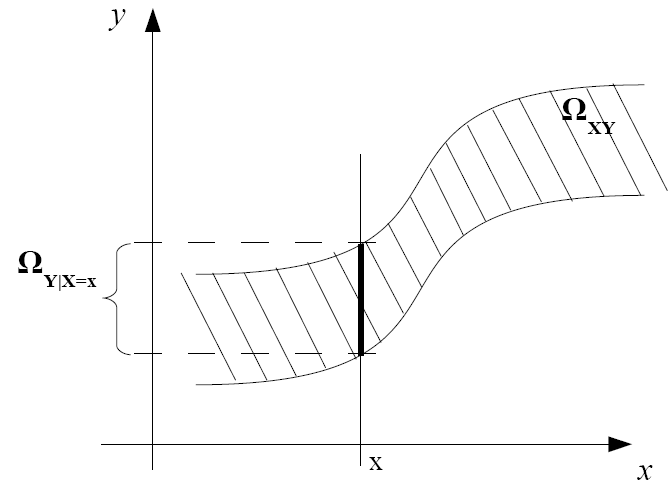
\includegraphics[width=5cm]{estejem.png} \qquad 
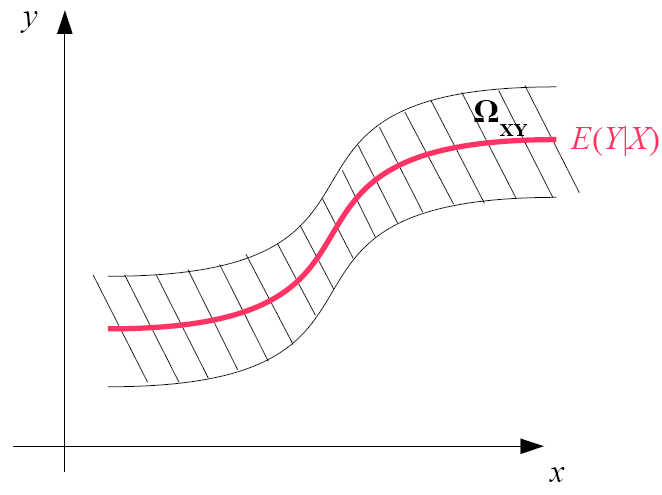
\includegraphics[width=5cm]{estesp.png} \qquad 
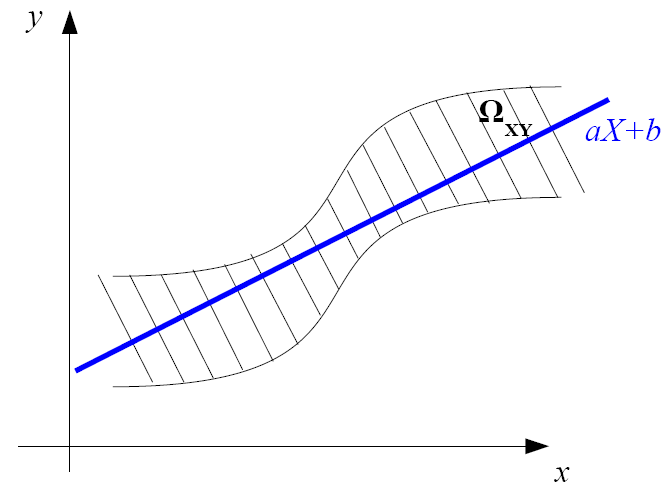
\includegraphics[width=5cm]{estlin.png}
\caption{Esquerra: exemple de conjunt de valors possibles de $Y$ donat un valor $X=x$. Centre: millor estimaci\'o de $Y$
a partir dels valors de $X$. Dreta:  millor estimaci\'o lineal de $Y$ a partir dels valors de $X$.
Suposam distribuci\'o uniforme de la probabilitat.}
\end{figure}
 
\vskip 0.2 cm
\noindent
Per mesurar la qualitat de l'estimaci\'o utilitzam
la ra\'o de correlaci\'o. La \textbf{ra\'o de correlaci\'o de $Y$ sobre $X$} es defineix com:
\[
\eta_{Y|X}^2=\frac{\mathrm{Var}(Y^*)}{\mathrm{Var}(Y)}
\]

\noindent
Propietats: 
\begin{itemize}
\item $0 \leq \eta_{Y|X}^2 \leq 1$

El valor $1$ significa que l'estimaci\'o \'es perfecta ($Y^* = Y$ per a tot $x$).

\item si $Y^* = E(Y|X)$ llavors $\eta_{Y|X}^2=1-\frac{\mathrm{ECM}}{\mathrm{Var}(Y)}$
\end{itemize}

\newpage
\begin{exemple}
Estimau la traject\`oria lineal d'un avi\'o de guerra a partir de les posicions de caiguda
de les bombes que ha llan\c{c}at. Les coordenades dels impactes es mostren en la taula seg\"uent:
\begin{center}
\begin{tabular}{c|c}
$x$ & $y$ \\ \hline
0.5 & 10 \\
0.4 & 12 \\
0.9 & 14 \\
1.5 & 11 \\
1.8 & 14.5 \\
2 & 17 \\
2.5 & 13 \\
\end{tabular}
$\qquad \qquad \qquad$
\begin{tabular}{c|c}
$x$ & $y$ \\ \hline
3 & 16 \\
3.2 & 17 \\
3.4 & 14 \\
3.7 & 16 \\
4 & 19 \\
4.5 & 17 \\
5.5 & 21
\end{tabular}
\end{center}
\end{exemple}



\vskip 0.2 cm
\begin{exemple}
(Exercici 24).
$E(Y|X)$ \'es la funci\'o $g(X)$ que ``millor''aproxima $Y$ on 
``millor'' indica que l'error quadr\`atic mitj\`a
$E\left((Y-g(X))^2\right)$ \'es m\'{\i}nim. Aquesta funci\'o de $X$
s'anomena la {\bf corba de regressi\'o de la mitjana de $Y$ sobre
$X$}. An\`alogament tenim la corba de regressi\'o de la mitjana de $X$
sobre $Y$. Determinau les corbes de regressi\'o de les mitjanes i
les rectes de regressi\'o lineal si
$(X,Y)$ est\`a distribu\"{\i}t uniformement en el triangle de
v\`ertexs (0,0), (1,0) i (1,2).
\end{exemple}


\vskip 1.5cm
\noindent
Problemes proposats: 17ef, 25a, 16d


\end{document}
